\section{Experiments}

We have measured the overhead of our OpenACC autocompare implementation to demonstrate its usability.
We used three of the SPEC ACCEL v1.2 benchmarks, using the \emph{test} dataset.
In each case, the program has an outer time step loop containing the main computation.
The times shown are in seconds, and these are officially SPEC \emph{estimates}, since they were not run in the SPEC harness.
The host machine was a 6-core Intel Haswell (core i7-5820K) with a 3.30GHz clock, with an NVIDIA Tesla Kepler K40c GPU.
We used the default autocompare options, but set a relative tolerance.
The values shown in Table~\ref{res1} are:
\begin{itemize}
\item Time (seconds) to run the test data sequentially on the CPU.
\item Time (seconds) to run the test data in parallel on the GPU.
\item Time (seconds) to run the test data on both CPU and GPU using the autocompare feature.
\item Number of variables or arrays compared.
\item Number of data items compared.
\end{itemize}



\begin{figure*}[t]
    \centering
    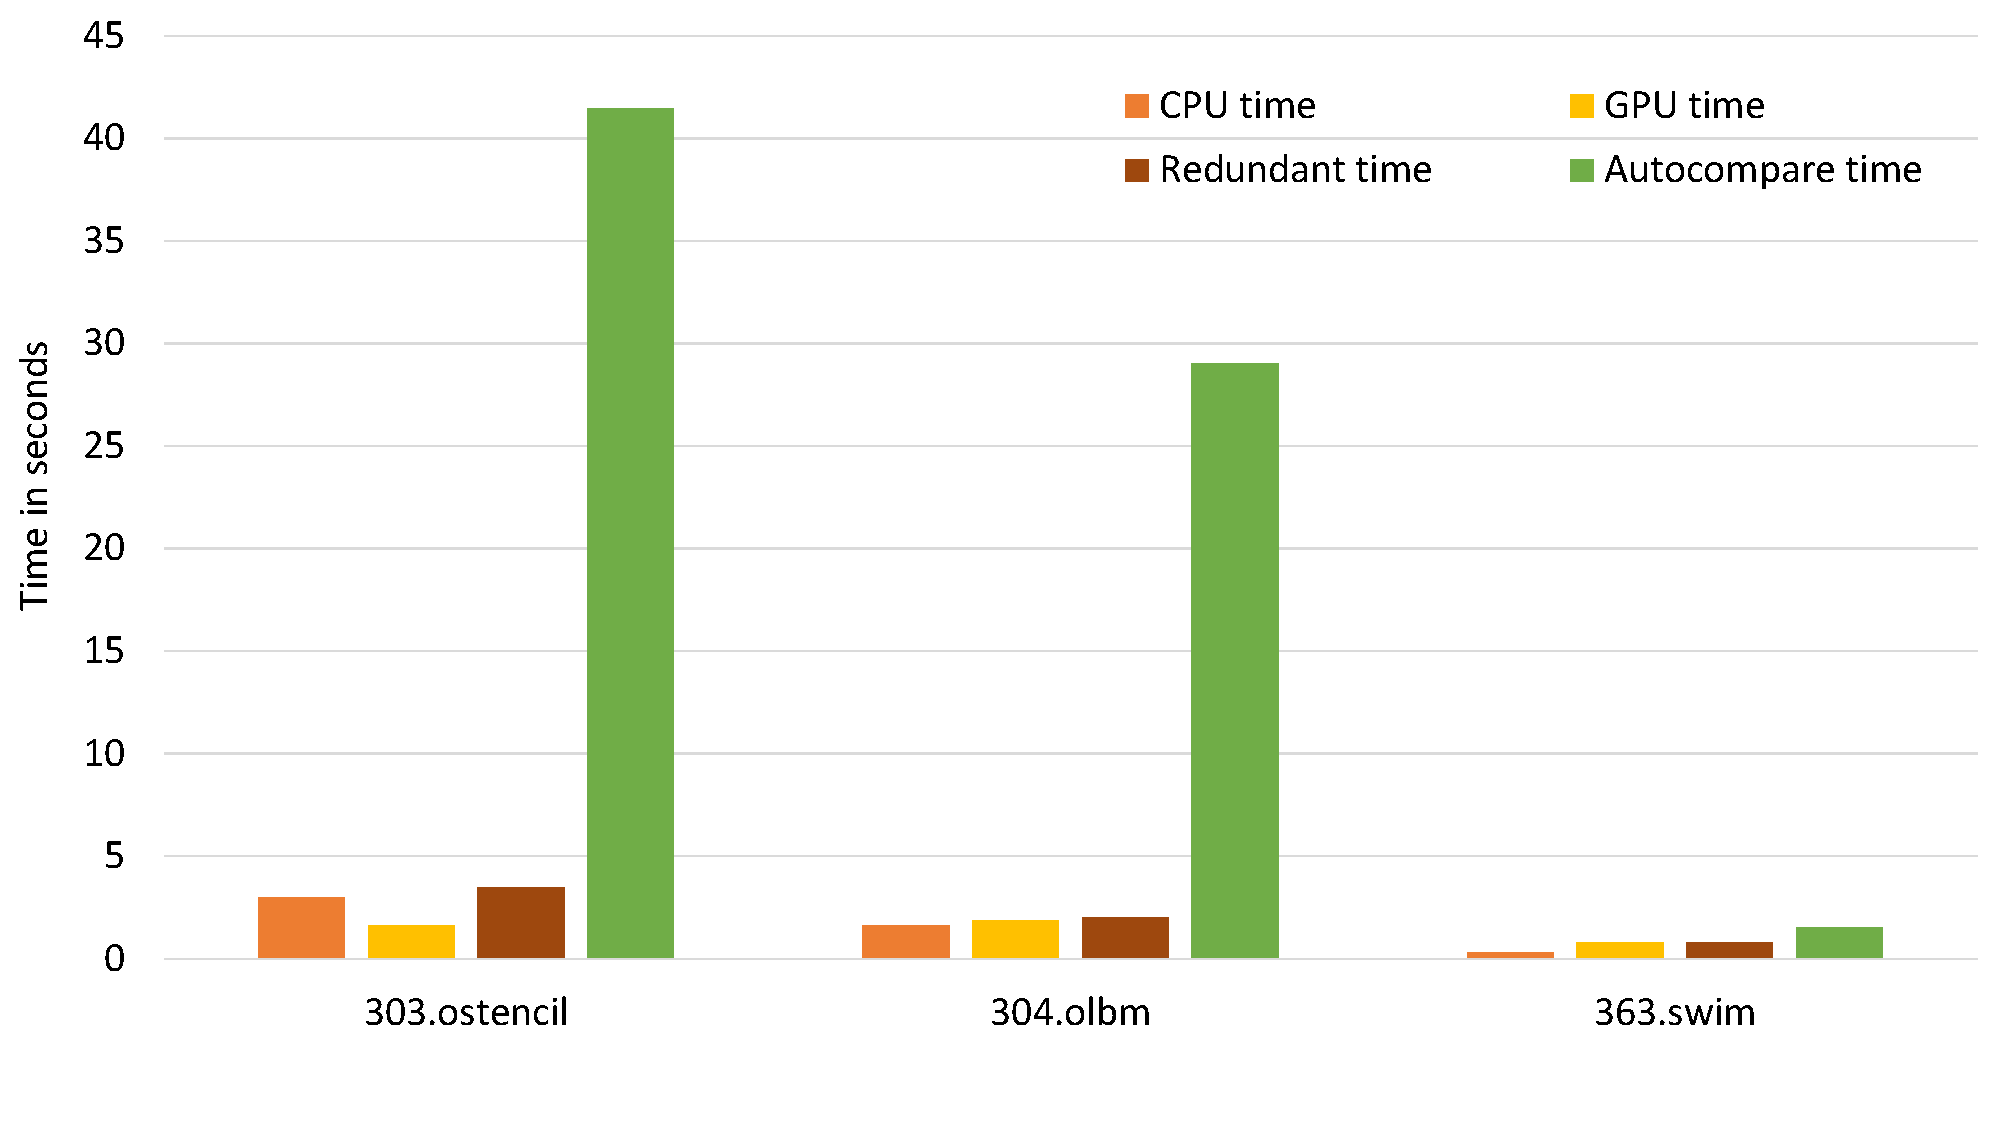
\includegraphics [width=\linewidth] {Table1.pdf}
    \caption{Results showing overhead of OpenACC autocompare.}
    \label{fig:sle_fiure}
\end{figure*}




\begin{table}
\begin{center}
\begin{tabular}{rrrl}
\hline
303.ostencil & 304.olbm & 363.swim & \\
\hline
 3.01 &  1.61 & 0.33 & CPU time \\
 1.61 &  1.85 & 0.78 & GPU time\\
41.46 & 29.05 & 1.53 & autocompare time \\
202 & 61 & 258 & variables and arrays compared \\
3,388,997,632 & 1,586,800,000 & 67,897,602 & items compared \\
\hline
\end{tabular}
\end{center}
\caption{Results showing overhead of OpenACC autocompare.}
\label{res1}
\end{table}

The two costs of the autocompare feature are running the program on both CPU and GPU, and downloading and comparing the values.
Even compared to sequential CPU time, the overhead is significant, and seems directly related to the number of words or elements compared.
However, using this feature to find where a GPU computation diverges moves the cost from the programmer to the computer, so it could be invaluable regardless of the overhead.
One side note: the \emph{test} datasets are relatively small.
Even so, we had to set the relative tolerance to avoid the comparisons detecting differences due to different summation accumulation order.
